% 02_previous_work_first.tex

Most work in deep learning for CSI estimation focuses on different neural network architectures, training frameworks, or hyperparameter tuning. Such works treat the real and imaginary elements of $\mathbf H$ as separate channels similar to color channels in images. The normalization method used in these works is typically the same -- the extrema (i.e., the minimum and the maximum) of the real and imaginary channels are used to perform minmax scaling over the entire dataset. For the scalar $H_n(i,j)$, the minmax-scaled version of this element is
\begin{align*}
	H_{n,\text{minmax}}(i,j) &= \frac{H_n(i,j)-H_{\text{min}}}{H_{\text{max}}-H_{\text{min}}},
\end{align*}
for $n \in [1,\dots,N]$ given a dataset of $N$ samples and $i/j$ indexing the rows/columns of the CSI matrices. The resulting samples are cast to the range $[0,1]$.

For image data, minmax normalization results in each image's color channels scaled to the range $[0,1]$. The resulting distribution for each color channel is typically satisfactory for image tasks, as the variance is not much smaller than the range of the normalized data (see Fig.~\ref{fig:imagenet_dist}).

However, for CSI matrices, minmax normalization is applied to the real and imaginary channels of each element. For typical channel models and parameters, the distribution of channel elements (see Fig.~\ref{fig:cost_indoor_dist}) tends to have much lower variance than that of image data. This smaller variance can be explained by the difference in the datasets' ranges -- while the channels in image data (e.g., ImageNet) assume integer values between $[0,255]$, the channels in CSI data (e.g., COST2100) assume floating point values smaller than $10^{-3}$.

\begin{figure}[htb]
	\centering
	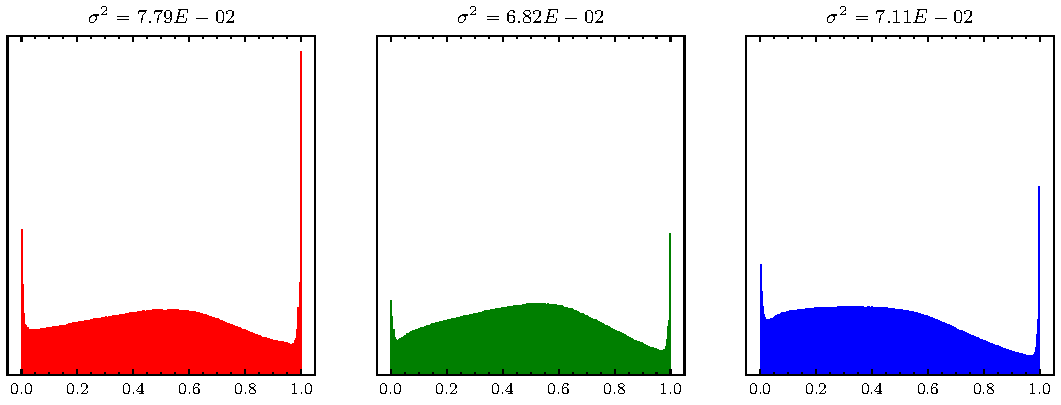
\includegraphics[width=.9\textwidth]{imagenet_rgb_dist.pdf}
	\medskip
	\caption{Distribution and variance of minmax-normalized ImageNet color channels ($N=50000$) images.}
	\label{fig:imagenet_dist}
\end{figure}

\begin{figure}[htb]
	\centering
	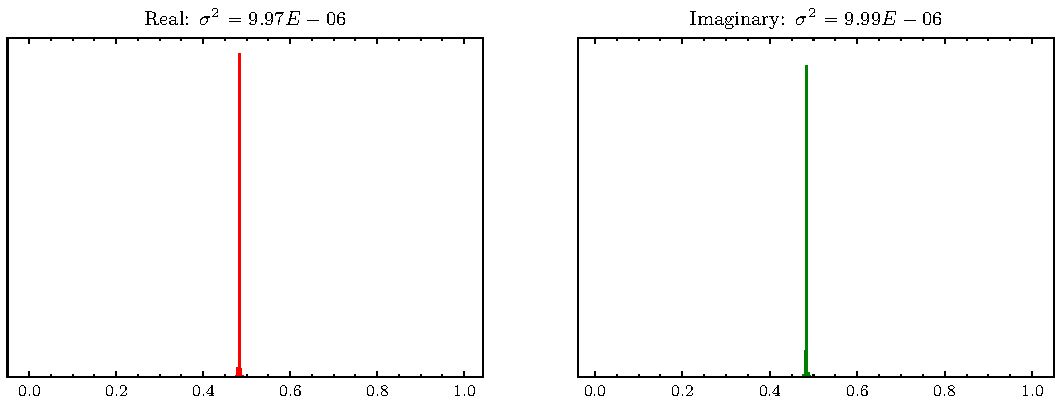
\includegraphics[width=.9\textwidth]{cost2100_indoor_dist.pdf}
	\medskip
	\caption{Distribution and variance of minmax-normalized COST2100 real/imaginary channels ($N=99000$) images.}
	\label{fig:cost_indoor_dist}
\end{figure}

\subsection{Related Work}

Several works have investigated normalization techniques for deep learning such as batch normalization \cite{ref:ioffe2015batch}, instance normalization \cite{ref:huang2017instance}, layer normalization \cite{ref:ba2016layer}, and group normalization \cite{ref:wu2018group}. These normalization techniques scale the outputs of latent layers in neural networks, which helps to solve the problem of covariate shift \cite{ref:ioffe2015batch} where the mean and variance of changes between subsequent layers of the network.

Other works have studied normalization of the network's inputs. A number of works have investigated adaptive normalization techniques for time series estimation tasks \cite{ref:ogasawara2010adaptive, ref:nayak2014impact, ref:shao2015self}. In \cite{ref:passalis2019dain}, the authors proposed a trainable input network which learns to shift, scale, and filter the unnormalized data while training the target network for a time series prediction task.

\subsection{Methods}

Here, we discuss our work in spherical normalization (Section~\ref{sect:sph_norm_method}) and our optimized network architecture (Section~\ref{sect:csinet_pro}) \cite{ref:liu2020sphnet}.

\subsubsection{Spherical Normalization}
\label{sect:sph_norm_method}
Rather than apply minmax normalization, which is adversely impacted by outliers, we propose spherical normalization. Before describing spherical normalization in detail, consider z-score normalization. Given a random variable, $x$, with mean $\mu$ and standard deviation $\sigma$. The z-score normalized version of this random variable is given as
\begin{align}
	z &= \frac{x - \mu}{\sigma^2}. \label{eq:zscore}
\end{align}
Assuming $x$ is normally distributed, the resulting random variable, $z$, is a standard normal distribution such that $z \sim \mathcal N(0,1)$. Inspired by $z$-score normalization, we seek a normalization scheme which adjusts the range of each channel sample. Under spherical normalization, each sample in the dataset is scaled by its power. Denote the $k$-th downlink CSI matrix of the dataset as $\mathbf H_d^k$. The spherically normalized version of the downlink CSI is given as
% TODO: Does this make sense? "For CSI matrices, we could choose to scale each element by it's mean and by the inverse covariance matrix."
\begin{align}
	\mathbf{\check H}_d^n &= \frac{\mathbf H_d^n}{\|\mathbf H_d^n\|}. \label{eq:sph-intro}
\end{align}
Observe that (\ref{eq:sph-intro}) is similar to (\ref{eq:zscore}) without the mean shift in the numerator\footnote{Since the mean of COST2100 data is $\approx 10^{-10}$, we can safely ignore this mean shift in spherical normalization.} and with the power term of each CSI sample rather than the variance of the entire distribution. After applying (\ref{eq:sph-intro}) to each sample, minmax scaling is applied to the entire dataset. The resulting dataset under spherical normalization can exhibit a larger variance than the same dataset under minmax scaling (compare Fig.~\ref{fig:cost_indoor_sph_dist} with Fig.~\ref{fig:cost_indoor_dist}). 
\begin{figure}[htb]
	\centering
	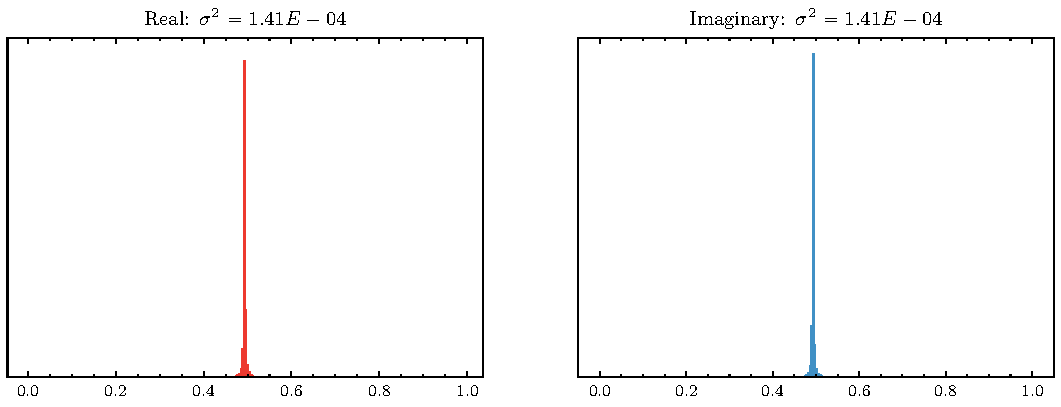
\includegraphics[width=.9\textwidth]{cost2100_indoor_sph_dist.pdf}
	\medskip
	\caption{Distribution and variance of COST2100 real/imaginary channels under spherical normalization ($N=99000$) images.}
	\label{fig:cost_indoor_sph_dist}
\end{figure}

Beyond desirable properties in the input distribution, spherical normalization also results in an objective function which is better matched with the evaluation criterion. Neural networks for CSI estimation are optimized using the mean-squared error loss,
\begin{align} 
	\text{MSE}&=\frac 1N \sum_{k=1}^N\Arrowvert\mathbf H_k - \hat{\mathbf H}_k\Arrowvert^2, \label{eq:mse}
\end{align}
while channel state reconstruction accuracy is measured in terms of normalized mean-squared error,
\begin{align} 
	\text{NMSE}&=\frac 1N \sum_{k=1}^N\frac{\Arrowvert\mathbf H_k - \hat{\mathbf H}_k\Arrowvert^2}{\Arrowvert\mathbf H_k\Arrowvert^2}. \label{eq:nmse}
\end{align}
Observe that when the $\mathbf H_k \; (\hat{\mathbf H}_k)$ in (\ref{eq:mse}) is replaced with $\check{\mathbf H}_k \; (\hat{\check{\mathbf H}}_k)$, we have
\begin{align*} 
	\frac 1N \sum_{k=1}^N\Arrowvert\check{\mathbf H}_k - \hat{\check{\mathbf H}}_k\Arrowvert^2&= \frac 1N \sum_{k=1}^N\left\Arrowvert \frac{\mathbf H_k}{\Arrowvert\mathbf H_k\Arrowvert^2} - \frac{\hat{\mathbf H}_k}{\Arrowvert\mathbf H_k\Arrowvert^2}\right\Arrowvert^2 \\
	&= \frac 1N \sum_{k=1}^N\frac{\Arrowvert\mathbf H_k - \hat{\mathbf H}_k\Arrowvert^2}{\Arrowvert\mathbf H_k\Arrowvert^2},
\end{align*}
which is equivalent to (\ref{eq:nmse}). Thus, a neural network optimized with MSE as the loss function and trained using spherically normalized data is in fact being optimized with respect to NMSE of the original data.

\subsubsection{CsiNet-Pro}
\label{sect:csinet_pro}

In \cite{ref:liu2020sphnet}, we proposed a network with larger convolutional kernels and no residual connections called CsiNet-Pro. Large kernels (e.g., $(7\times 7)$ in CsiNet-Pro) allow the network to capture features corresponding to larger delay spreads than comparatively small kernels (e.g., $(3\times 3)$ in CsiNet \cite{ref:csinet}).
\begin{figure}[htb]
  \centering
  {
    \fontsize{1pt}{1pt}
    \def\svgwidth{1.0\columnwidth}
    \input{../images/csinet-pro.pdf_tex}
  }
  % 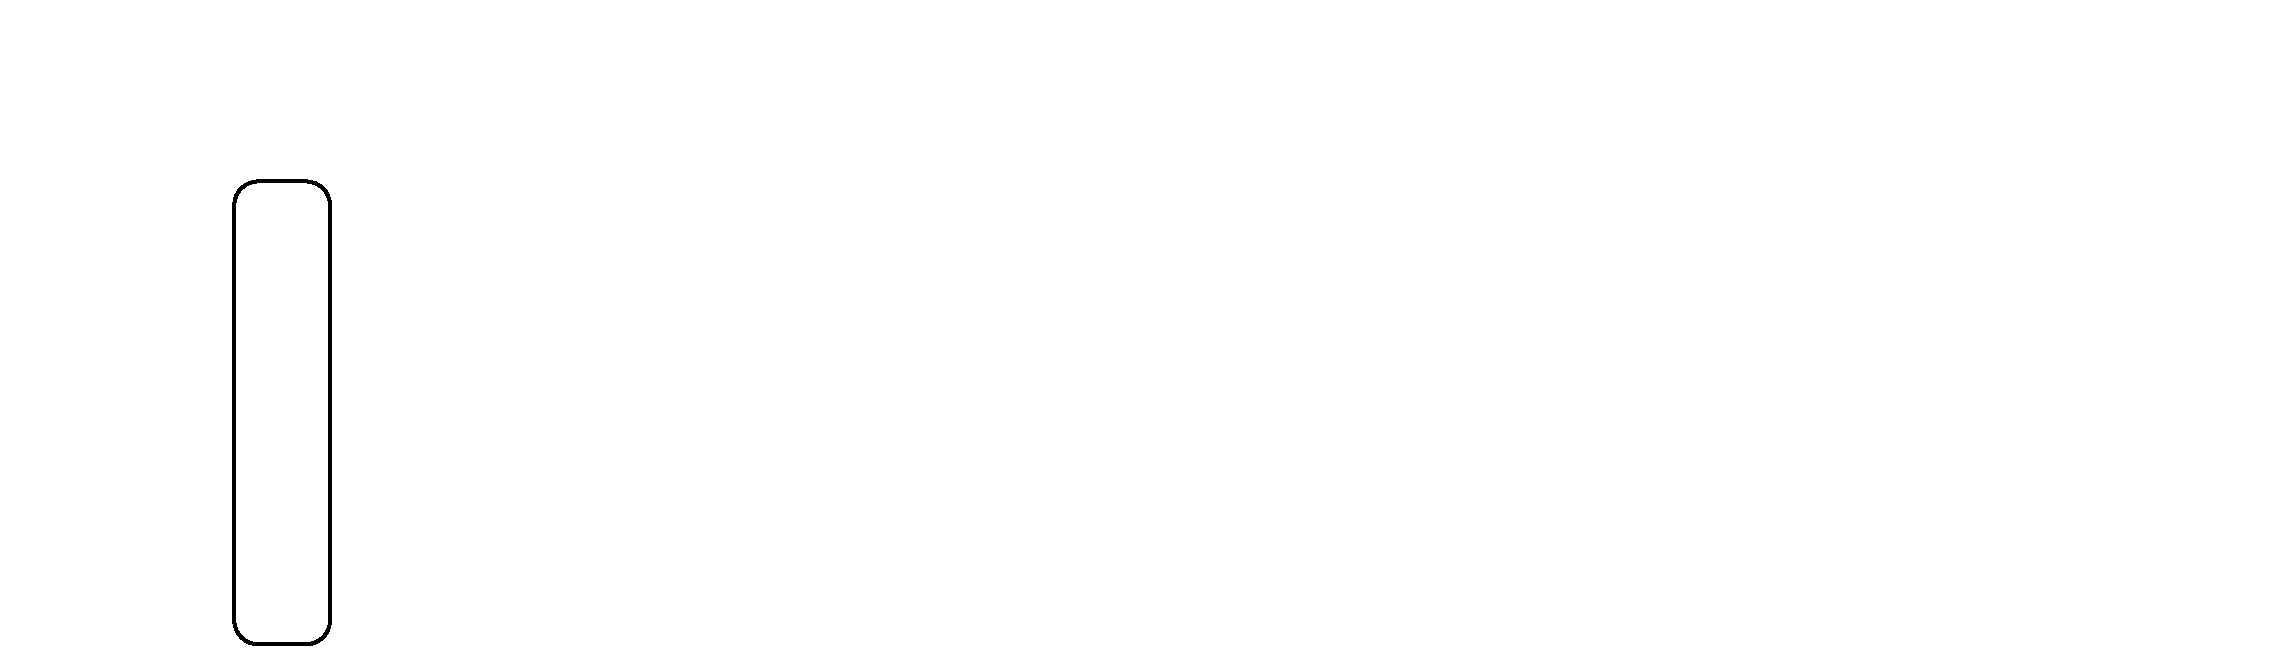
\includegraphics[width=.9\textwidth]{csinet-pro.pdf}
  % \medskip
  \caption{SphNet -- CsiNetPro architecture with Spherical Normalization.}
  \label{fig:sphnet-arch}
\end{figure}

\subsection{Results}
Training on spherically normalized data and optimizing with respect to NMSE can yield better accuracy. Fig.~\ref{fig:nmse_slot1} demonstrates this improvement for CsiNet and CsiNet-Pro on the COST2100 dataset. CsiNet and CsiNet-Pro are trained with minmax normalization while CsiNet-Sph and SphNet are trained with spherical normalization. % For both networks, the number of 

\begin{figure}[!hbtp] \centering 
	\begin{subfigure}[t]{.45\textwidth}
		\centering
		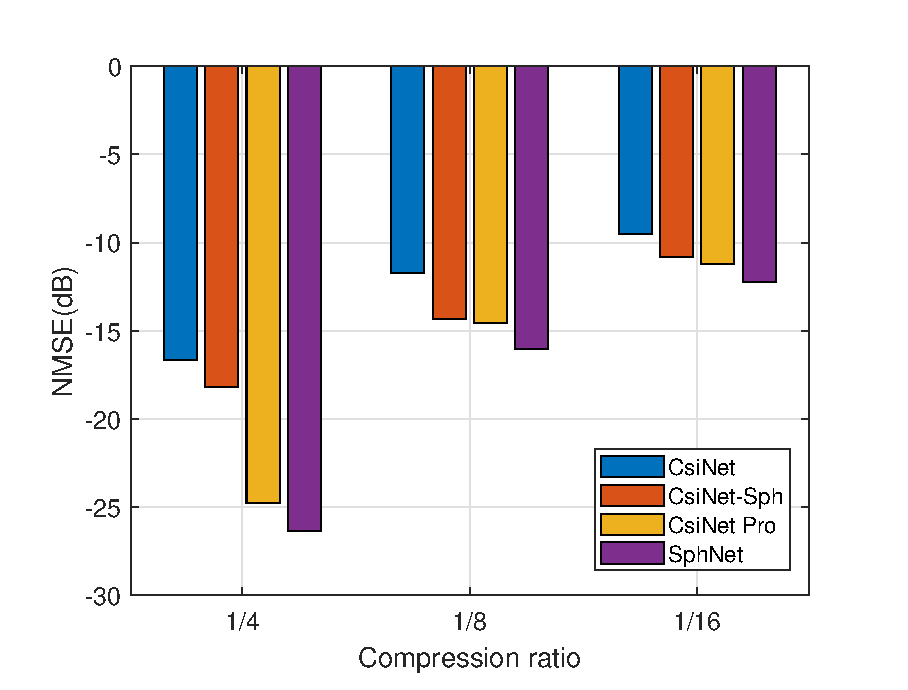
\includegraphics[width=\linewidth]{nmse_slot1_indoor.eps}
		\caption{Indoor}
		\label{fig:slot1_indoor} 
	\end{subfigure}
	\begin{subfigure}[t]{.45\textwidth}
		\centering
		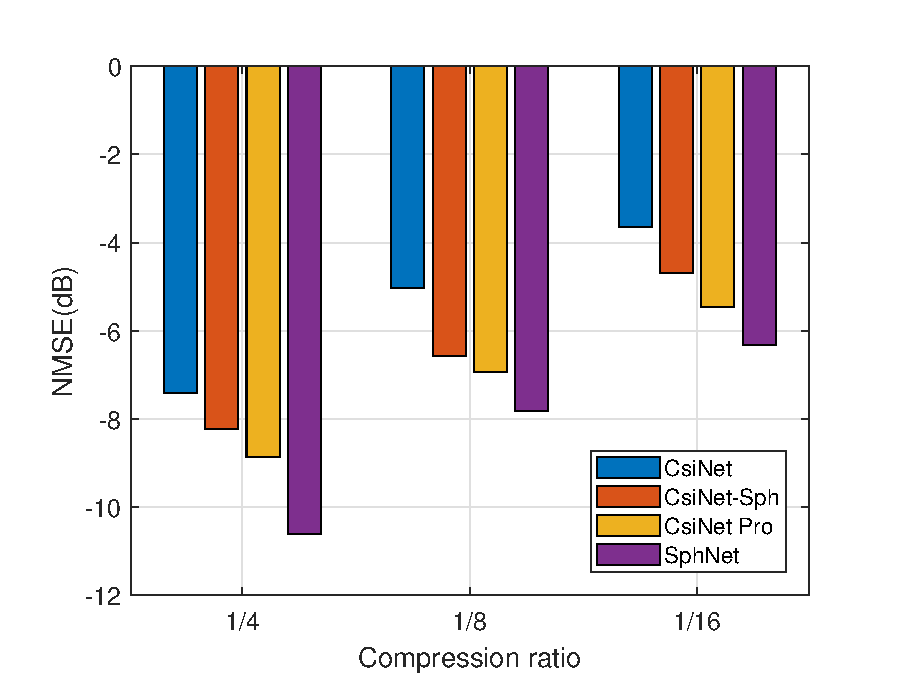
\includegraphics[width=\linewidth]{nmse_slot1_outdoor.eps}
		\caption{Outdoor}
		\label{fig:slot1_outdoor} 
	\end{subfigure}
	\caption{Reconstruction error for CsiNet \cite{ref:csinet} and CsiNet Pro with and without spherical normalization. SphNet combines CsiNet Pro with spherical normalization \cite{ref:liu2020sphnet}.}
	\label{fig:nmse_slot1} 
\end{figure}
